\section{Resumo}


\begin{figure}[h!]
    \centering
    \label{fig1}
    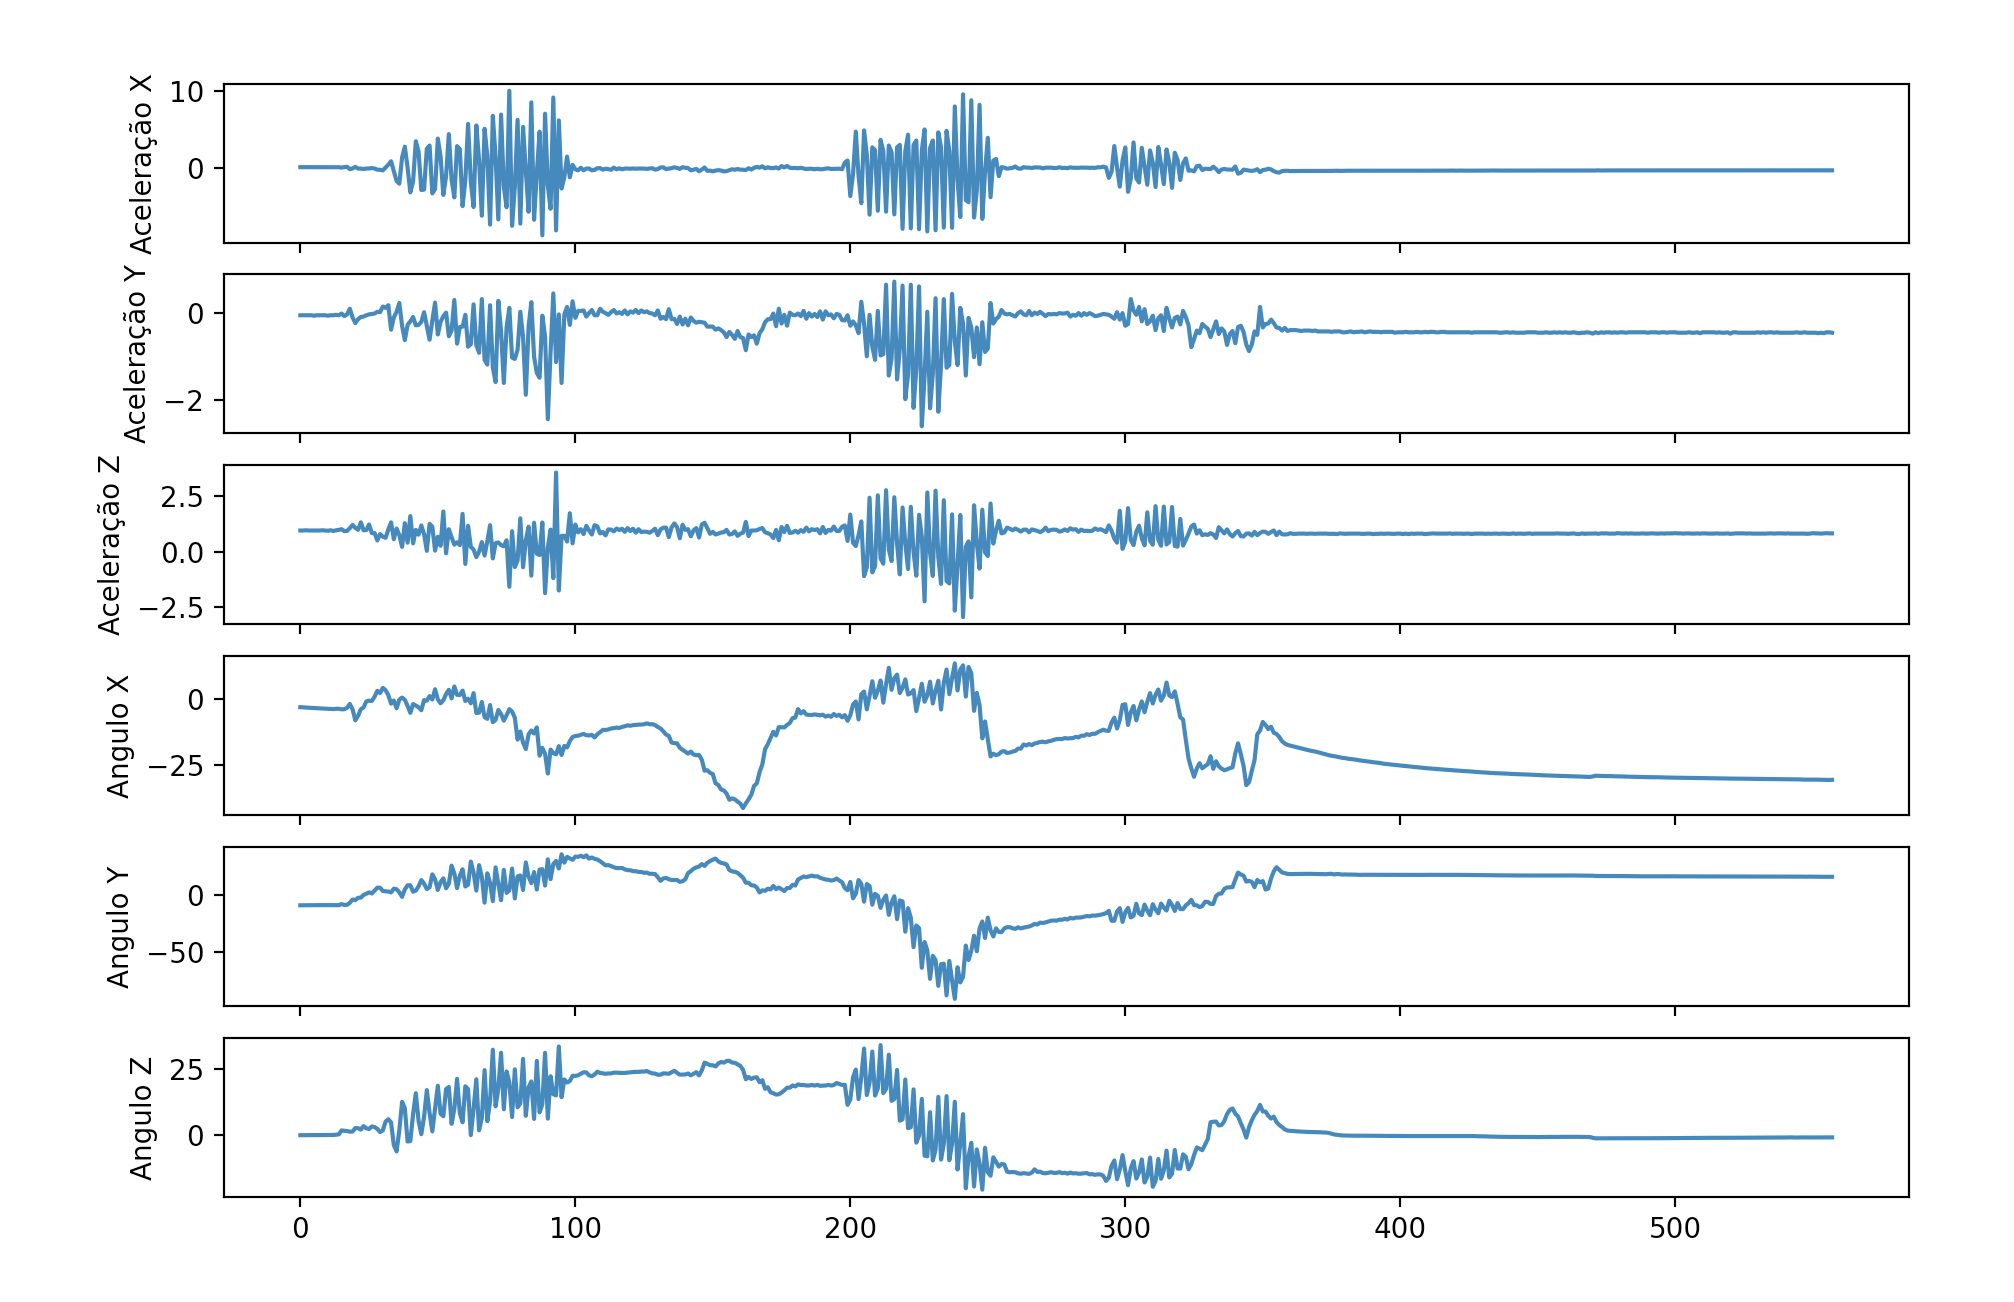
\includegraphics[scale=0.2]{images/VibracaoX.png}
    \caption{VibracaoX}
\end{figure}

\begin{figure}[h!]
    \centering
    \label{fig2}
    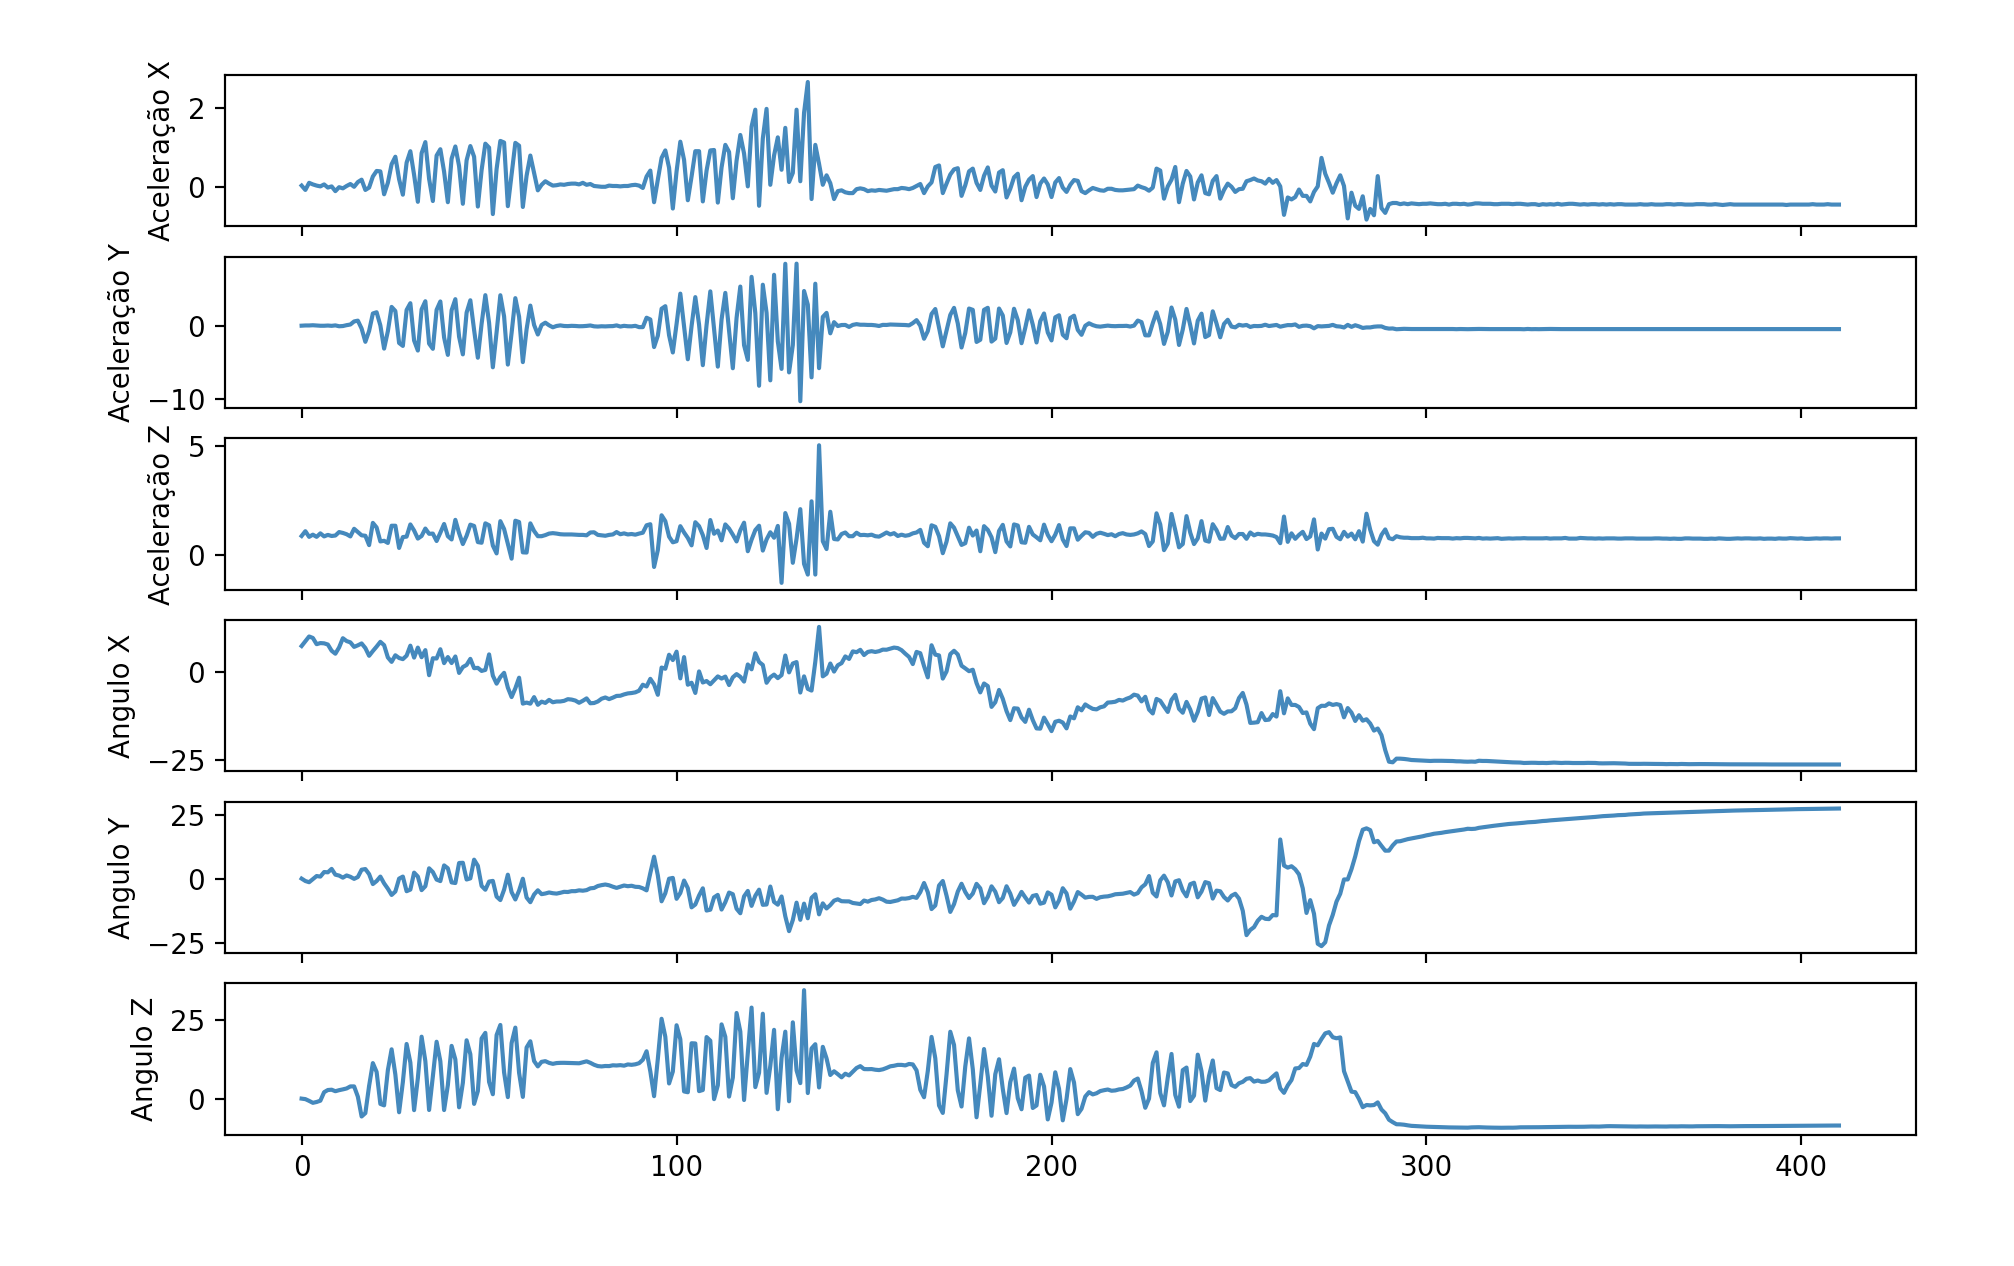
\includegraphics[scale=0.2]{images/VibracaoY.png}
    \caption{VibracaoY}
\end{figure}

\begin{figure}[h!]
    \centering
    \label{fig3}
    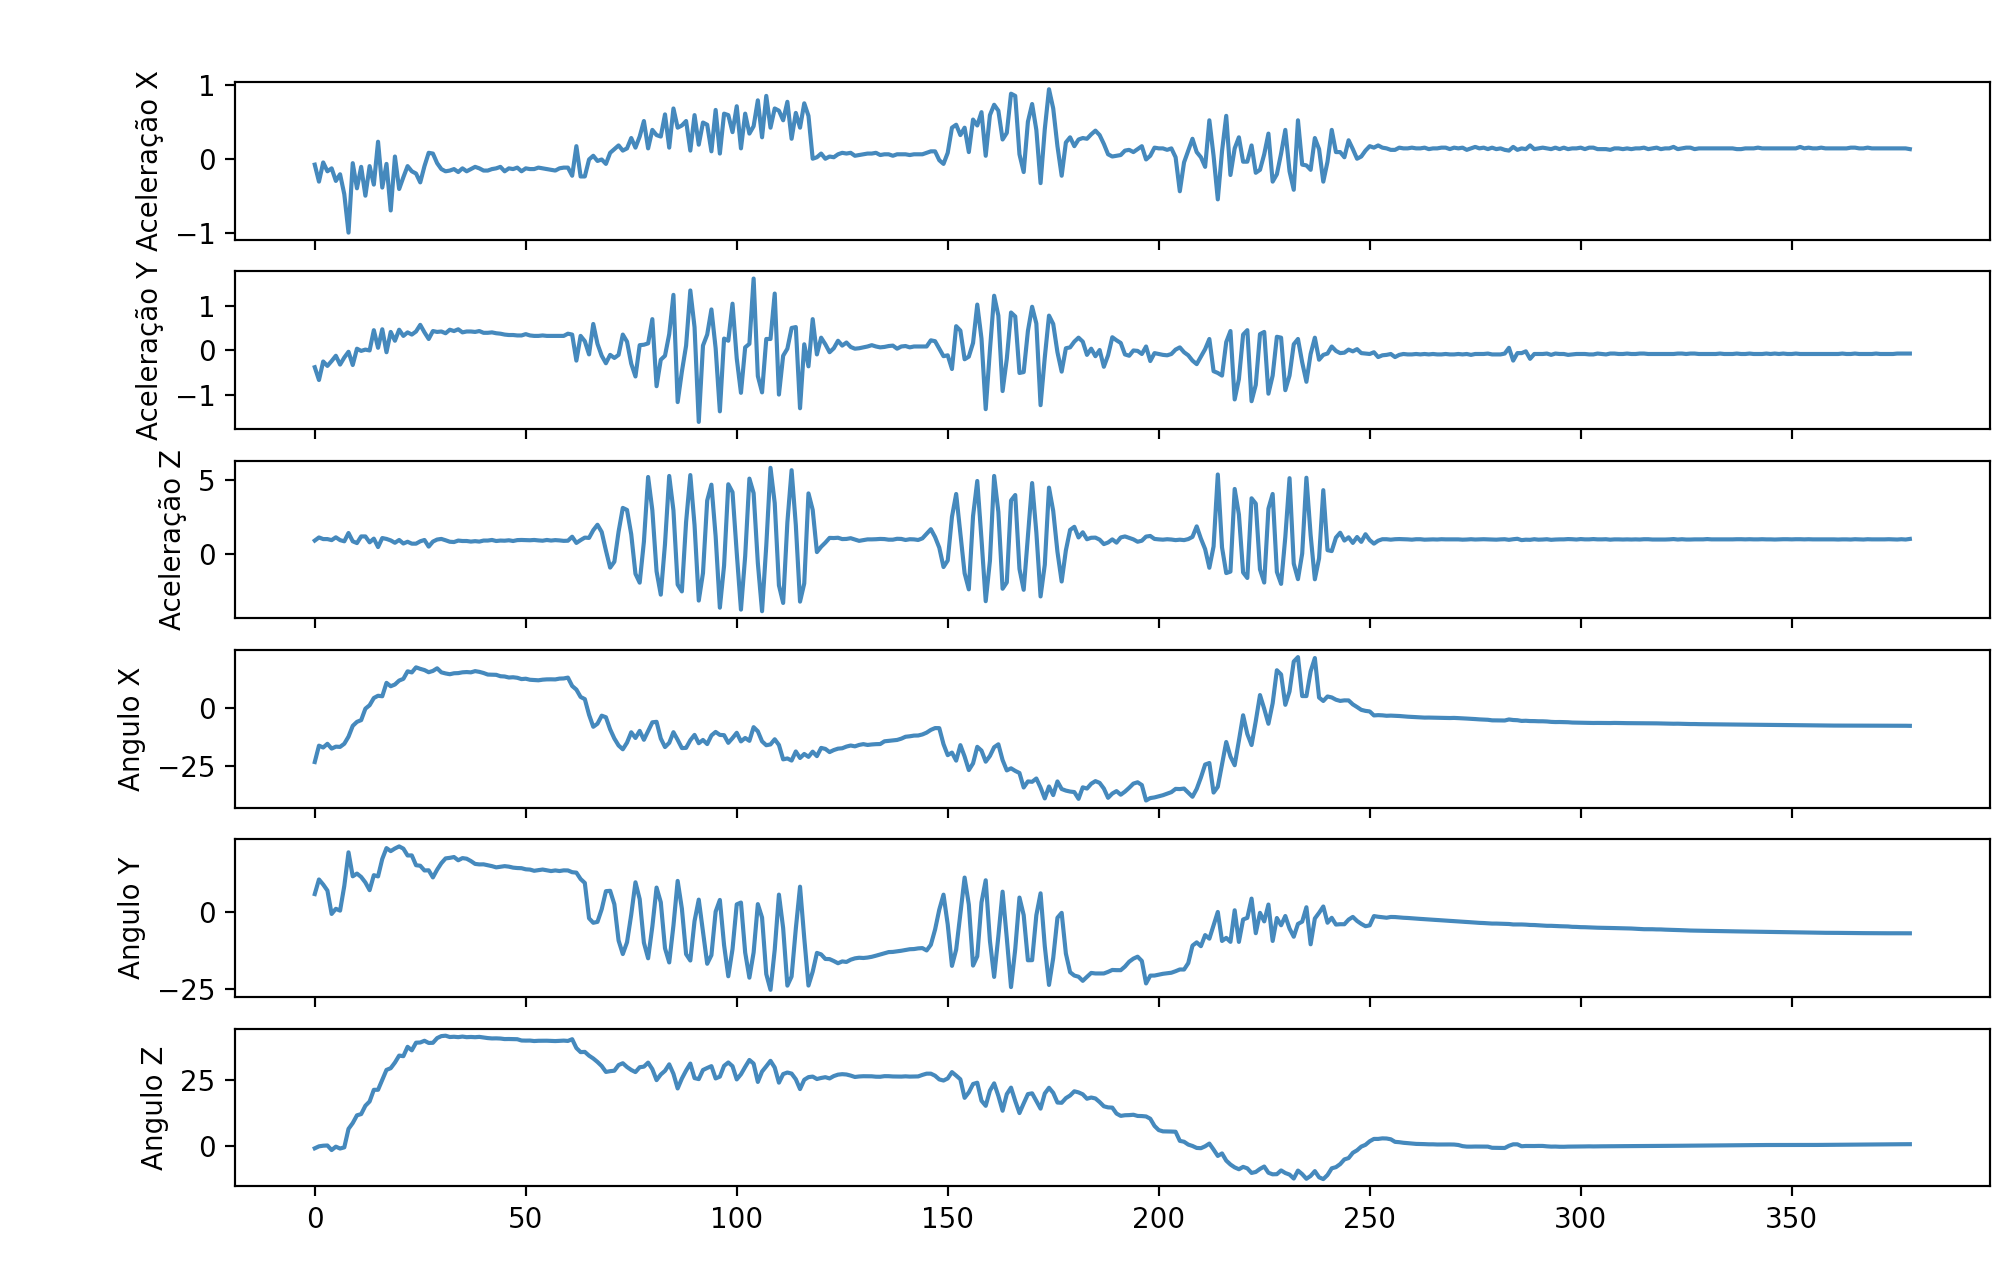
\includegraphics[scale=0.2]{images/VibracaoZ.png}
    \caption{VibracaoZ}
\end{figure}

\begin{figure}[h!]
    \centering
    \label{fig4}
    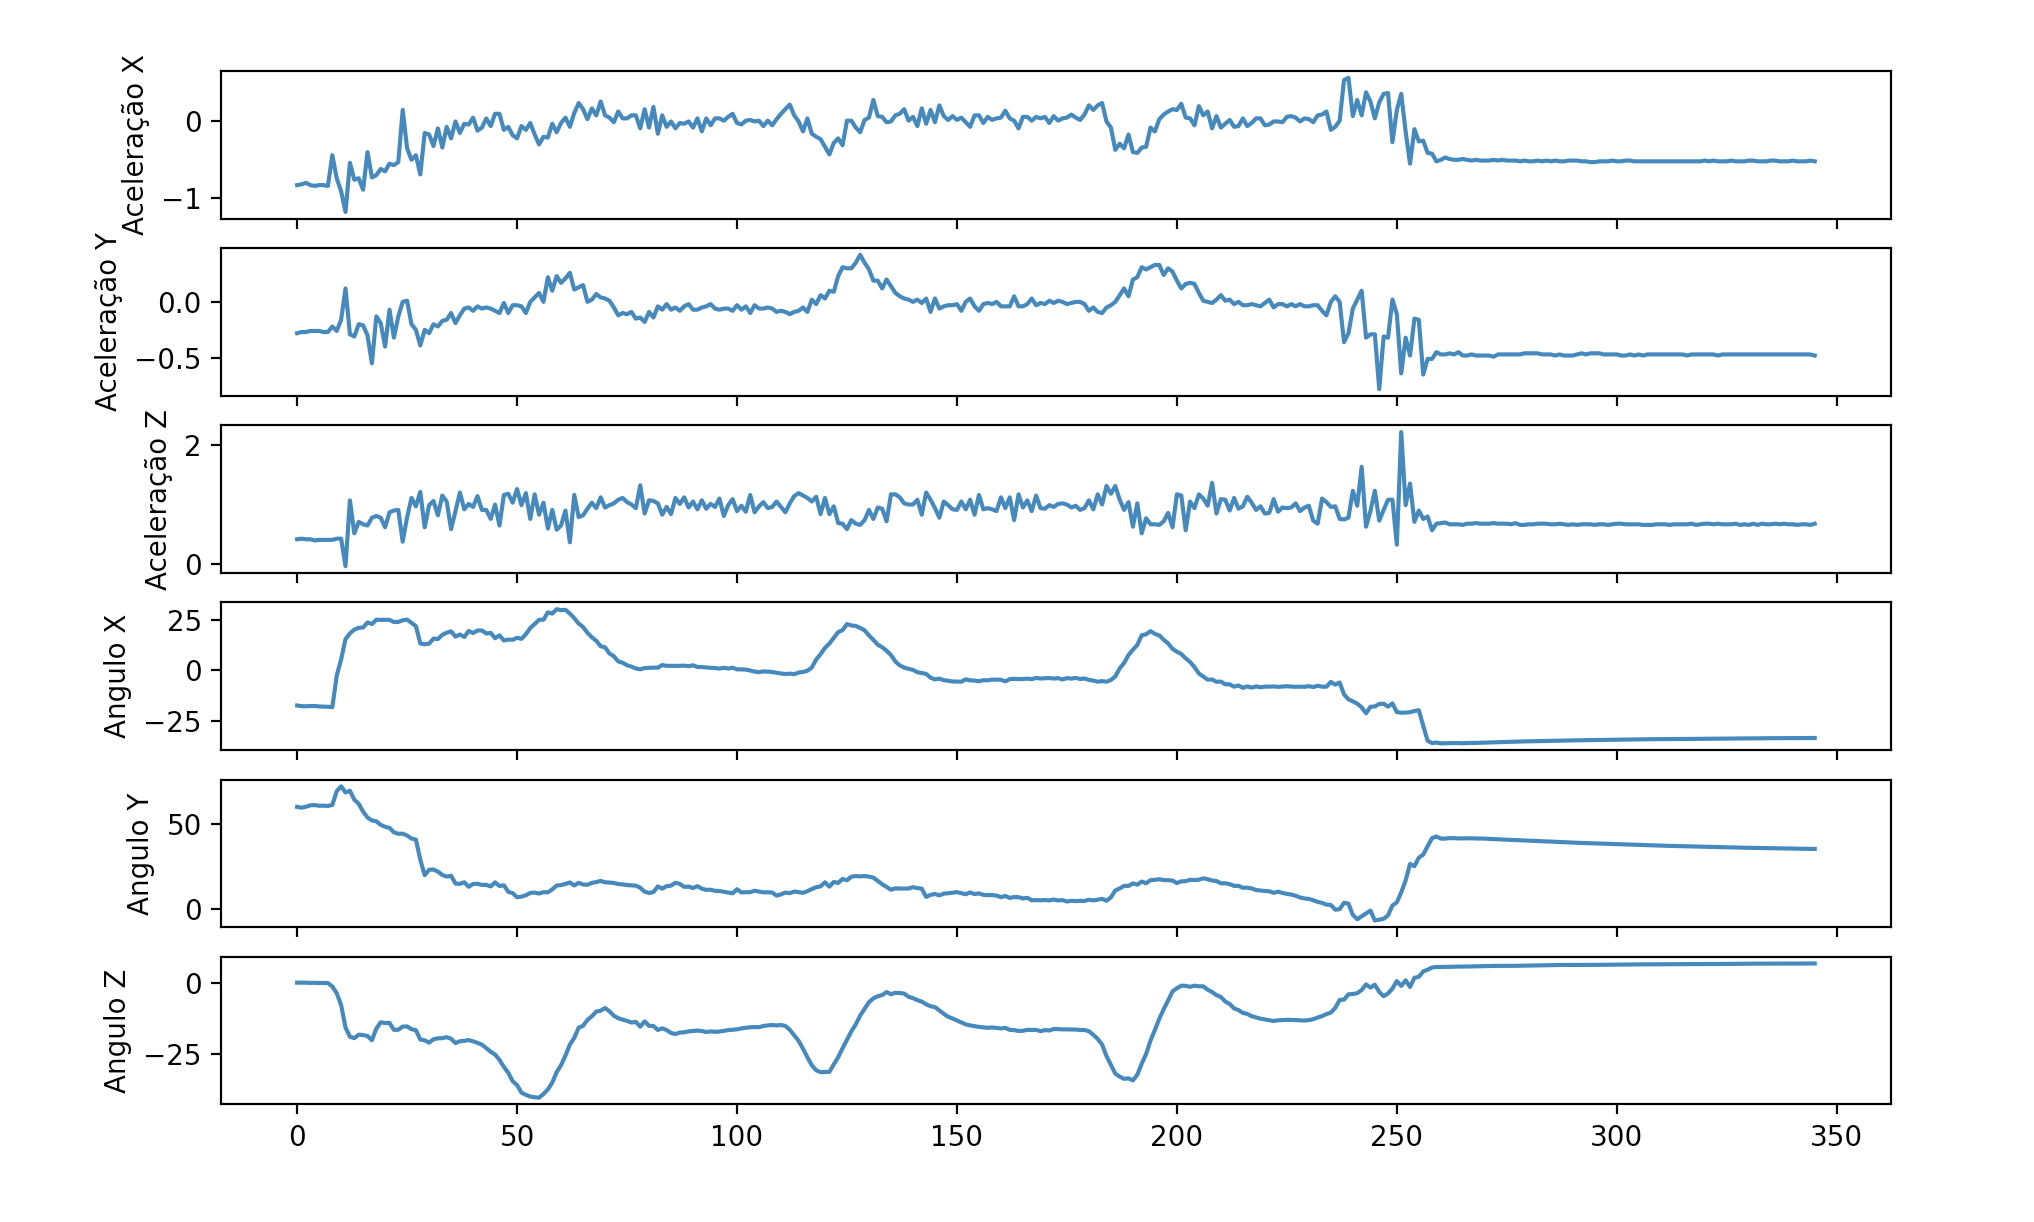
\includegraphics[scale=0.2]{images/CirculoZ.png}
    \caption{CirculoZ}
\end{figure}
\begin{figure}[h!]
    \centering
    \label{fig5}
    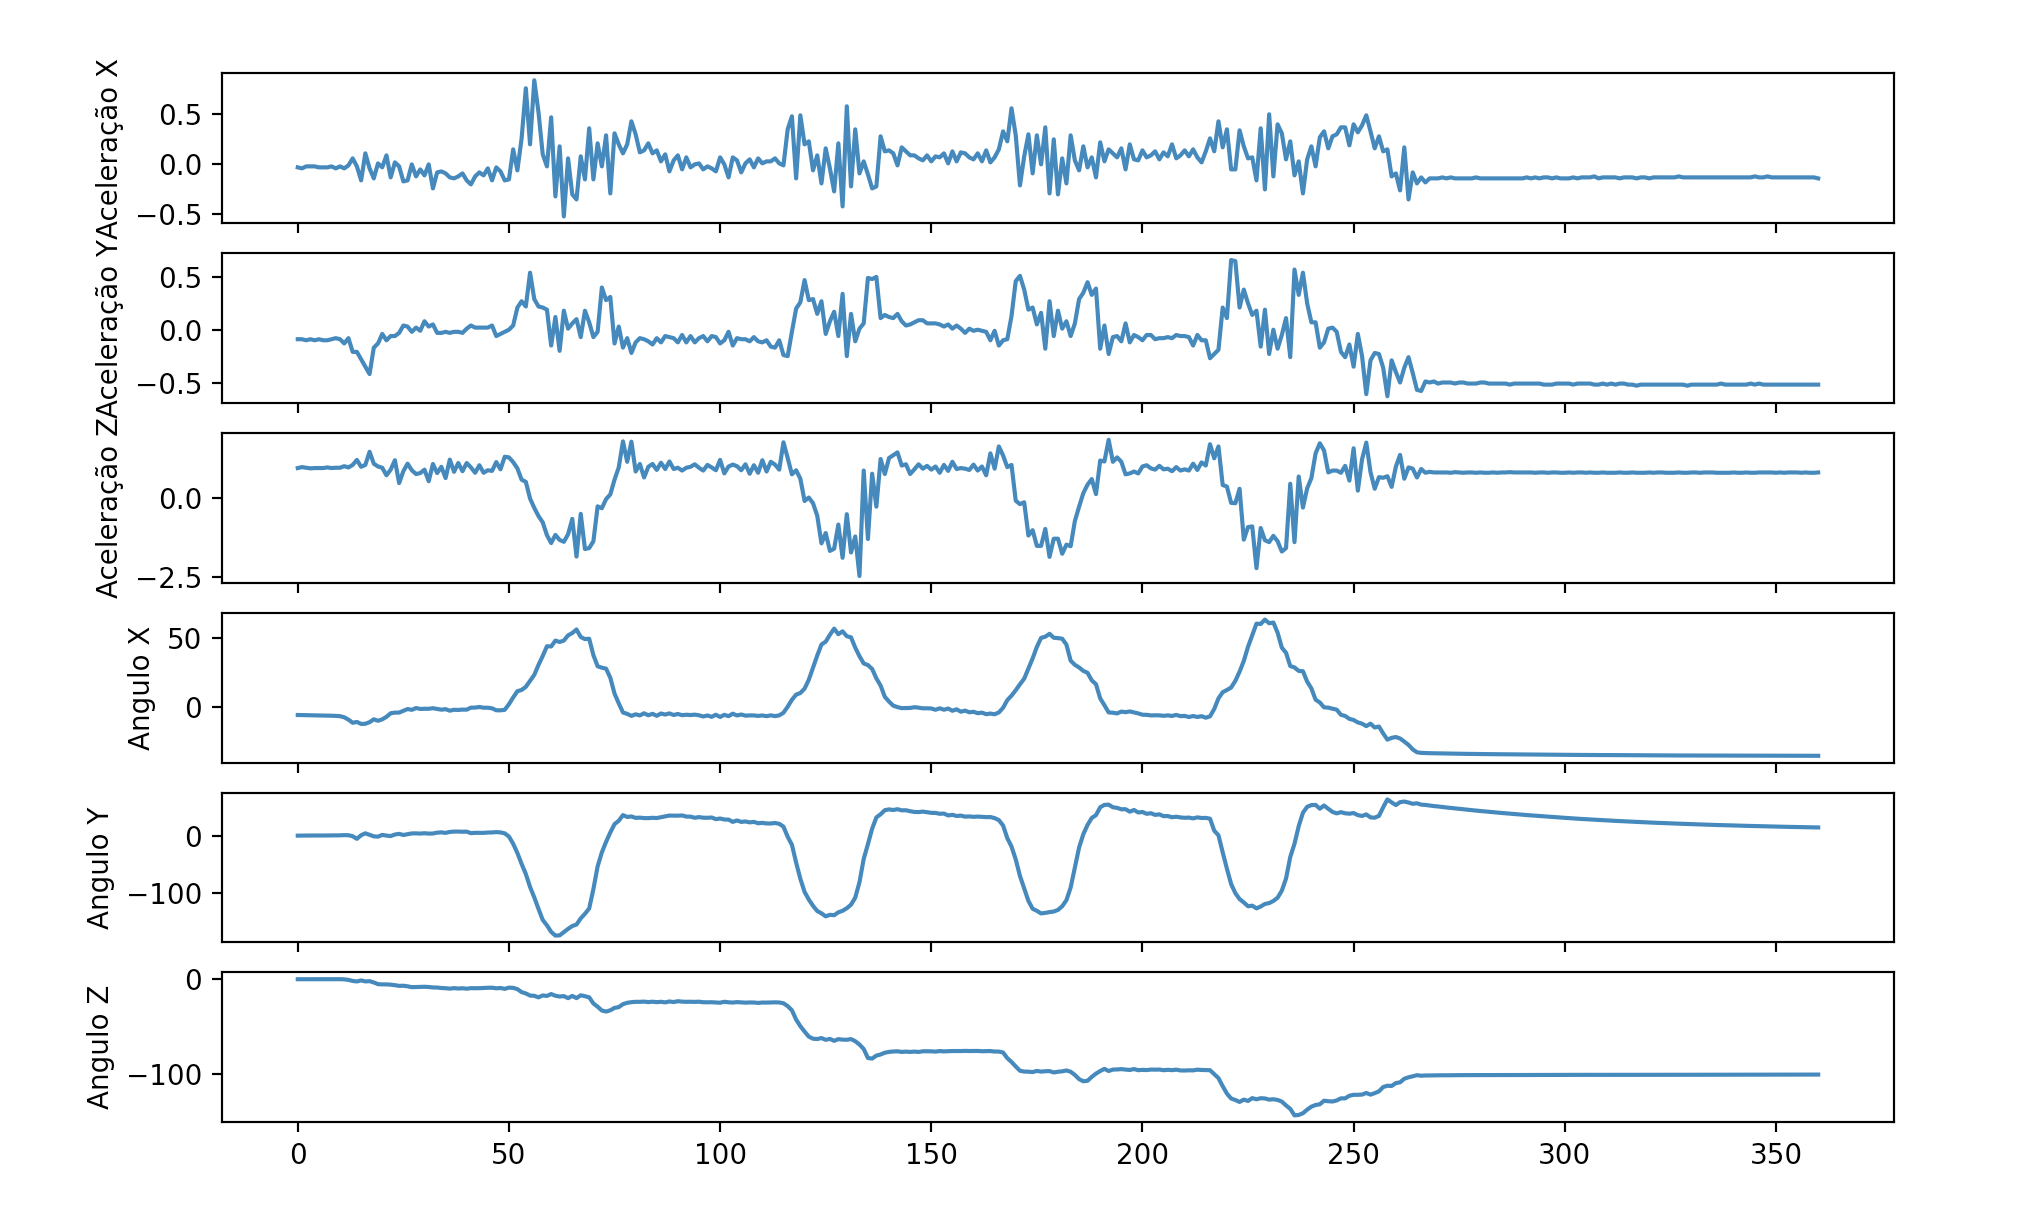
\includegraphics[scale=0.2]{images/GiraeVoltaY.png}
    \caption{GiraeVoltaY}
\end{figure}



Seguindo os site https://towardsdatascience.com/feature-engineering-on-time-series-data-transforming-signal-data-of-a-smartphone-accelerometer-for-72cbe34b8a60
temos a funcionalidade de feature engineering.

Nesse extrai um código em python capaz de calcular:

1. mean
2. standard deviation
3. average absolute deviation
4. minimum value
5. maximum value
6. difference of maximum and minimum values
7. median
8. median absolute deviation
9. interquartile range
10. negative values count
11. positive values count
12. number of values above mean
13. number of peaks
14. skewness
15. kurtosis
16. energy
17. average resultant acceleration
18. signal magnitude area

Desses irei fazer uma analise com os dados:
Usarei apenas mean, median, number of peaks, energy, signal magnitude area, avg resultant

